% Provenance (never printed): cycle 4 SVT, "La planete Terre": earthquakes,
% faults, seismic waves and their recording, magnitude and intensity, the
% link with plate boundaries; natural hazards (tsunamis) and prevention; see
% sources/book1/PROVENANCE.md. Book 1, grade 7, chapter 3.
% Vocabulary guard: P and S waves are named in prose only (they were named in
% g6.4, defined in Book 2 g11); "sediment" not before g7.4; "intensity" is
% always the earthquake's (homograph with physics: linker STOP list).
\chapter{Os terremotos}\label{ch:g7:earthquakes}

Na manhã de 26~de~dezembro~de~2004, embaixo do \omterm{def:g2:water-on-earth:ocean}{mar}, ao largo da ponta
noroeste de Sumatra, na Indonésia, as \omterm{def:g3:stones-pebbles-sand:rock}{rochas} se romperam ao longo de uma
\omterm{def:g7:earthquakes:fault}{falha}: foi um dos maiores \omterm{def:g4:volcanoes-earthquakes-first-look:earthquake}{terremotos} já medidos. No \omterm{def:g1:landscapes-around-us:water}{litoral} vizinho de
Sumatra, o \omterm{def:g2:water-on-earth:ocean}{mar} subiu em ondas de até \qty{51}{m} de altura, que avançaram
até \qty{5}{km} terra adentro. Nas horas seguintes, as ondas atravessaram
o \omterm{def:g2:water-on-earth:ocean}{oceano} Índico e atingiram os \omterm{def:g1:landscapes-around-us:water}{litorais} de quinze países, até a África.
Cerca de 230\,000 pessoas morreram. Na época, não havia nenhum sistema de
alerta no \omterm{def:g2:water-on-earth:ocean}{oceano} Índico.
% ledger: usgs:largest, nws:tsunami-2004

\begin{omfigure}
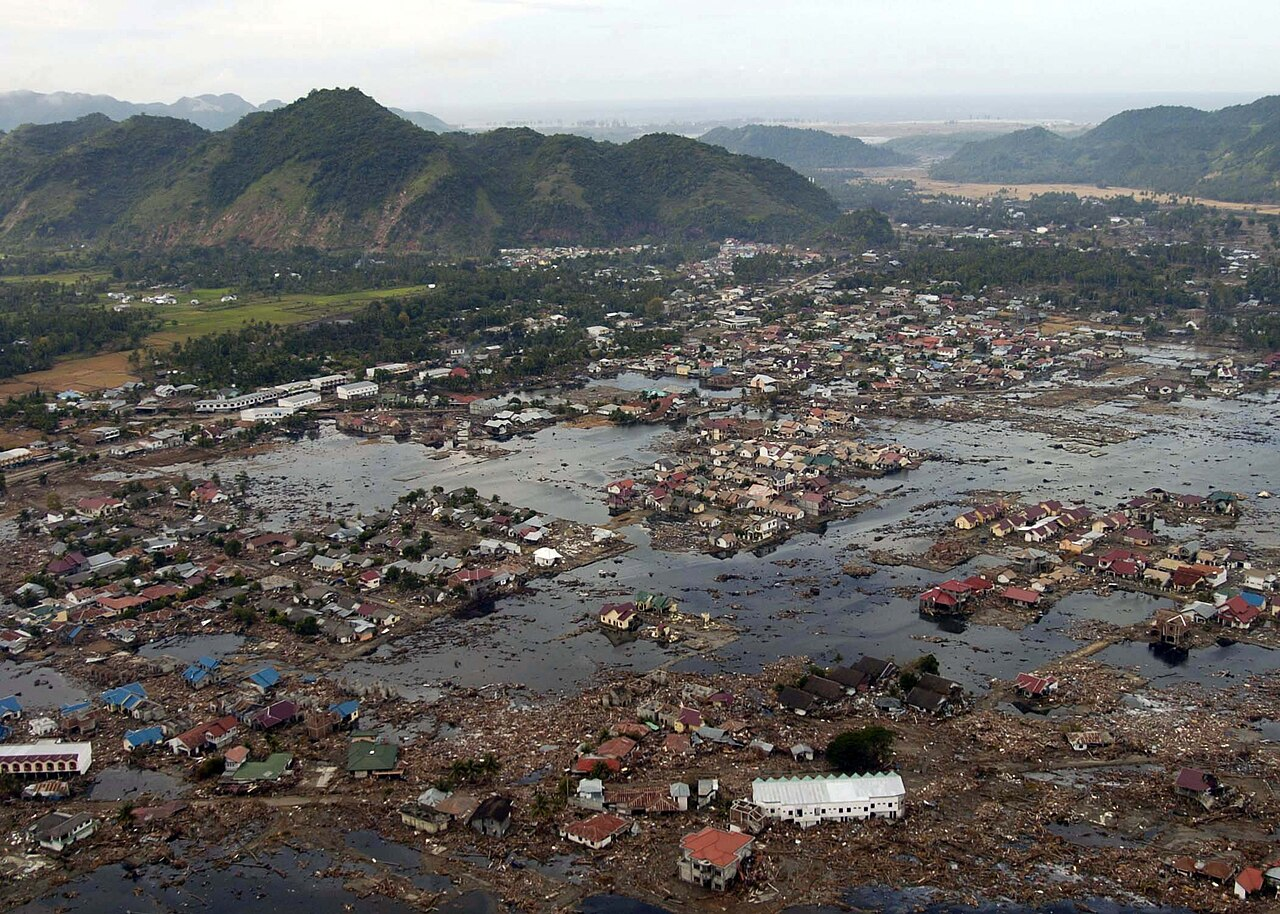
\includegraphics[width=0.78\linewidth]{images/book1/g7-tsunami-village.jpg}

{\small Uma aldeia perto do \omterm{def:g1:landscapes-around-us:water}{litoral} de Sumatra, uma semana depois do
\omterm{def:g7:earthquakes:tsunami}{tsunami} de 26~de~dezembro~de~2004. Fotografia da U.S. Navy por Philip~A.
McDaniel (domínio público, via Wikimedia Commons).}
% ledger: commons:tsunami-village
\label{fig:g7:earthquakes:tsunami-village}
\end{omfigure}

Como as \omterm{def:g3:stones-pebbles-sand:rock}{rochas} se rompem? Como os cientistas descobrem, em poucos minutos,
onde um \omterm{def:g4:volcanoes-earthquakes-first-look:earthquake}{terremoto} aconteceu e qual foi o seu tamanho? E por que o \omterm{def:g2:water-on-earth:ocean}{mar},
horas depois, subiu em \omterm{def:g1:landscapes-around-us:water}{litorais} onde ninguém tinha sentido nada?

\begin{recall}
Um \emph{\omterm{def:g4:volcanoes-earthquakes-first-look:earthquake}{terremoto}} é um tremor repentino do chão, causado por \omterm{def:g3:stones-pebbles-sand:rock}{rochas} que
se rompem e deslizam, bem fundo embaixo da terra
(\cref{ch:g4:volcanoes-earthquakes-first-look}). A casca externa da Terra
é feita de \omterm{def:g7:plate-tectonics:plate}{placas}, e 92~\% dos grandes \omterm{def:g4:volcanoes-earthquakes-first-look:earthquake}{terremotos} acontecem a menos de
\qty{300}{km} de um \omterm{def:g7:plate-tectonics:plate-boundary}{limite de placas} (\cref{ch:g7:plate-tectonics}).
Quando acontece um \omterm{def:g4:volcanoes-earthquakes-first-look:earthquake}{terremoto}, ondas viajam pelas \omterm{def:g3:stones-pebbles-sand:rock}{rochas} da Terra inteira:
um tipo mais rápido (as ondas~P) e um tipo mais lento (as ondas~S);
cronometrando-as, os cientistas descobriram o \omterm{def:g6:inside-the-earth:layers}{núcleo}
(\cref{ch:g6:inside-the-earth}).
\end{recall}

\section{Rochas que se rompem}

As \omterm{def:g7:plate-tectonics:plate}{placas} se movem alguns centímetros por ano, mas as suas bordas são
ásperas: elas ficam presas uma na outra enquanto o resto das \omterm{def:g7:plate-tectonics:plate}{placas}
continua se movendo. As \omterm{def:g3:stones-pebbles-sand:rock}{rochas} perto da borda se curvam um pouco, como uma
régua que você empurra pelas duas pontas, e acumulam energia. Quando o
empurrão finalmente vence o atrito, as \omterm{def:g3:stones-pebbles-sand:rock}{rochas} se soltam de uma vez e
deslizam: esse deslizamento repentino é o \omterm{def:g4:volcanoes-earthquakes-first-look:earthquake}{terremoto}.
% ledger: usgs:eq-basics

\begin{definition}[Falha]\label{def:g7:earthquakes:fault}
Uma \emph{falha}\index{falha} é uma ruptura nas \omterm{def:g3:stones-pebbles-sand:rock}{rochas} ao longo da qual os
dois blocos, um de cada lado, se deslocaram um em relação ao outro.
Durante um \omterm{def:g4:volcanoes-earthquakes-first-look:earthquake}{terremoto}, os blocos deslizam de repente ao longo da falha;
quanto maiores a falha e o deslizamento, maior o \omterm{def:g4:volcanoes-earthquakes-first-look:earthquake}{terremoto}.
\end{definition}

Um \omterm{def:g7:plate-tectonics:plate-boundary}{limite de placas} é feito de muitas \omterm{def:g7:earthquakes:fault}{falhas}, e a maioria dos \omterm{def:g4:volcanoes-earthquakes-first-look:earthquake}{terremotos}
do mundo acontece nelas. Mas também existem \omterm{def:g7:earthquakes:fault}{falhas} dentro das \omterm{def:g7:plate-tectonics:plate}{placas}, e
algumas delas também podem se romper. Quando uma grande \omterm{def:g7:earthquakes:fault}{falha} se rompe
perto da superfície, o deslizamento pode ser visto no chão: um degrau num
campo, uma estrada cortada em duas, uma cerca ou uma fileira de árvores
deslocada para o lado.
% ledger: usgs:eq-basics

\begin{omfigure}
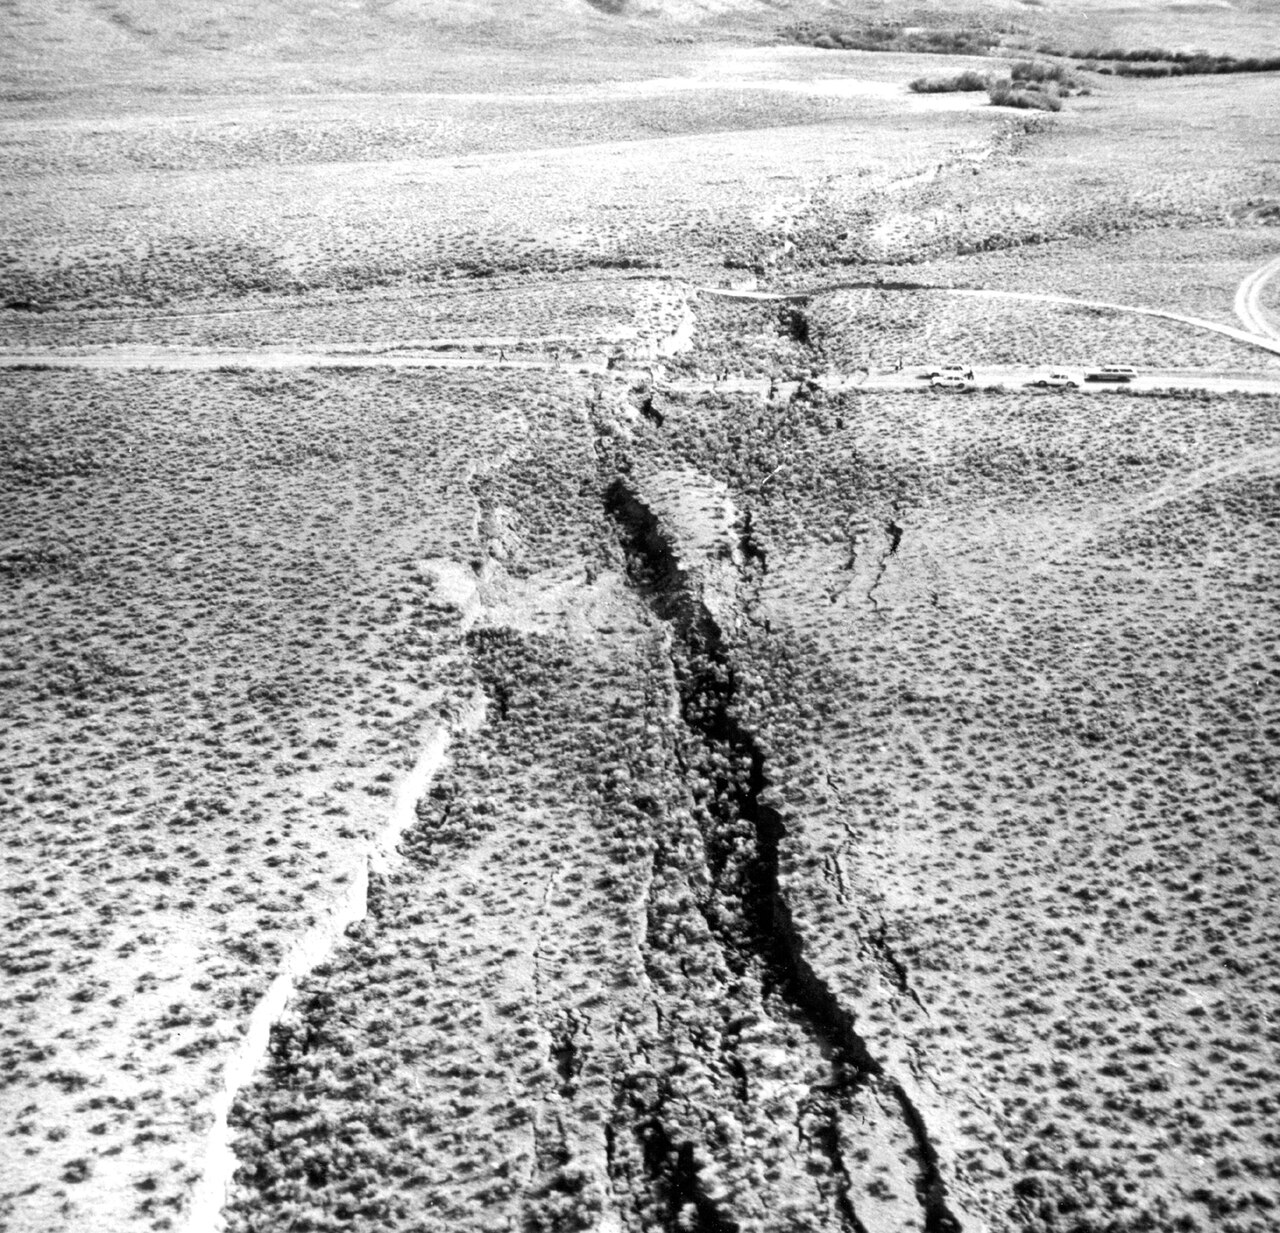
\includegraphics[width=0.62\linewidth]{images/book1/g7-borah-scarp.jpg}

{\small Degraus no chão deixados pelo \omterm{def:g4:volcanoes-earthquakes-first-look:earthquake}{terremoto} de Borah Peak, em 1983, em
Idaho (Estados Unidos), vistos do ar: ao longo da \omterm{def:g7:earthquakes:fault}{falha}, um lado desceu em
relação ao outro, e o degrau atravessa a estrada, no alto. Fotografia:
R.~E. Wallace, U.S. Geological Survey (domínio público, via Wikimedia
Commons).}
% ledger: commons:borah-scarp
\label{fig:g7:earthquakes:borah}
\end{omfigure}

\begin{definition}[Foco e epicentro]\label{def:g7:earthquakes:focus}
O \emph{foco}\index{foco} de um \omterm{def:g4:volcanoes-earthquakes-first-look:earthquake}{terremoto} é o lugar embaixo da terra, na
\omterm{def:g7:earthquakes:fault}{falha}, onde o deslizamento começa. O \emph{epicentro}\index{epicentro} é
o ponto da superfície da Terra que fica bem em cima do foco.
\end{definition}

O \omterm{def:g7:earthquakes:focus}{foco} muitas vezes fica a alguns quilômetros ou a algumas dezenas de
quilômetros de profundidade. Dos 7\,031 \omterm{def:g4:volcanoes-earthquakes-first-look:earthquake}{terremotos} de \omterm{def:g7:earthquakes:magnitude}{magnitude}~6 ou mais
registrados entre 1976 e 2025, 5\,561 --- 79~\% --- tiveram o seu \omterm{def:g7:earthquakes:focus}{foco} a
menos de \qty{70}{km} de profundidade. Mas 483 começaram a mais de
\qty{300}{km} de profundidade, e o mais profundo a \qty{688}{km}: esses
\omterm{def:g4:volcanoes-earthquakes-first-look:earthquake}{terremotos} profundos acontecem onde uma \omterm{def:g7:plate-tectonics:plate}{placa} afunda embaixo de outra,
dentro da \omterm{def:g7:plate-tectonics:plate}{placa} que afunda.
% ledger: data:usgs-comcat (figdata/grade-7/quake_counts.py, part depth)

Um grande \omterm{def:g4:volcanoes-earthquakes-first-look:earthquake}{terremoto} raramente vem sozinho. Muitas vezes, ele é seguido de
\omterm{def:g4:volcanoes-earthquakes-first-look:earthquake}{terremotos} menores no mesmo lugar, as \emph{réplicas}, durante semanas,
meses e até anos. Às vezes, \omterm{def:g4:volcanoes-earthquakes-first-look:earthquake}{terremotos} menores vêm antes dele, mas
ninguém consegue saber que eram avisos antes de o grande acontecer: os
cientistas não conseguem prever os \omterm{def:g4:volcanoes-earthquakes-first-look:earthquake}{terremotos}. Eles só conseguem dizer
que \omterm{def:g7:earthquakes:fault}{falhas} vão se romper de novo um dia, e ajudar as pessoas a se
preparar.
% ledger: usgs:eq-basics, usgs:seismograph

\begin{omfigure}
\begin{tikzpicture}[font=\small, x=1cm, y=1cm]
  % a block of crust seen in perspective: front face and top face
  \def\dx{2.2}\def\dy{1.3}
  % top surface: two blocks separated by the fault trace
  \fill[green!12] (0,0) -- (4.6,0) -- (4.6+\dx,\dy) -- (\dx,\dy) -- cycle;
  \fill[green!18] (4.6,0) -- (9,0) -- (9+\dx,\dy) -- (4.6+\dx,\dy) -- cycle;
  % front face
  \fill[brown!30] (0,0) -- (4.6,0) -- (3.4,-4) -- (0,-4) -- cycle;
  \fill[brown!40] (4.6,0) -- (9,0) -- (9,-4) -- (3.4,-4) -- cycle;
  % right face
  \fill[brown!22] (9,0) -- (9+\dx,\dy) -- (9+\dx,\dy-4) -- (9,-4) -- cycle;
  % fault plane on the front face and trace on top
  \draw[very thick, red!70!black] (4.6,0) -- (3.4,-4);
  \draw[very thick, red!70!black] (4.6,0) -- (4.6+\dx,\dy);
  % slip arrows
  \draw[-{Stealth[length=2.5mm]}, thick] (2.6,-0.35) -- (1.6,-0.35);
  \draw[-{Stealth[length=2.5mm]}, thick] (6.4,-0.35) -- (7.4,-0.35);
  \node[font=\footnotesize, anchor=south] at (2.1,-0.3) {bloco 1};
  \node[font=\footnotesize, anchor=south] at (6.9,-0.3) {bloco 2};
  % focus and waves
  \coordinate (F) at (3.95,-2.4);
  \foreach \r in {0.5,1.0,1.5,2.0}
    \draw[blue!60, dashed] (F) circle (\r);
  \fill[red!80!black] (F) circle (0.13);
  % epicentre: on the surface, straight above the focus (front edge of the top face)
  \coordinate (E) at (3.95,0);
  \draw[black!60, densely dotted, thick] (F) -- (E);
  \node[star, star points=5, star point ratio=2.4, fill=orange, draw=black, inner sep=1.4pt] at (E) {};
  % labels
  \node[anchor=west] at (9.5,-2.3) {foco};
  \draw[black!60] (9.45,-2.3) -- (4.1,-2.4);
  \node[anchor=south west] at (4.9,1.9) {epicentro};
  \draw[black!60] (4.95,1.95) -- (4.05,0.12);
  \node[anchor=south, red!70!black] at (6.8,1.3) {falha};
  \node[anchor=east, blue!60!black, align=right] at (-0.15,-2.6) {ondas que se espalham\\em todas as direções};
  \draw[blue!60, -{Stealth}] (-0.1,-2.6) -- (1.9,-2.5);
\end{tikzpicture}

{\small Uma \omterm{def:g7:earthquakes:fault}{falha}, o \omterm{def:g7:earthquakes:focus}{foco} e o \omterm{def:g7:earthquakes:focus}{epicentro} (um desenho, fora de escala). Os
dois blocos deslizam um ao lado do outro ao longo da \omterm{def:g7:earthquakes:fault}{falha} (em vermelho);
o deslizamento começa no \omterm{def:g7:earthquakes:focus}{foco}, e ondas se espalham a partir dele em todas
as direções, como as ondinhas num \omterm{def:g1:landscapes-around-us:water}{lago}. O \omterm{def:g7:earthquakes:focus}{epicentro} (a estrela) fica na
superfície, bem em cima do \omterm{def:g7:earthquakes:focus}{foco}.}
% ledger: usgs:eq-basics
\label{fig:g7:earthquakes:fault}
\end{omfigure}


\section{Registrar um terremoto}

\begin{definition}[Sismômetro e sismograma]\label{def:g7:earthquakes:seismometer}
Um \emph{sismômetro}\index{sismometro@sismômetro} é um instrumento que registra o
tremor do chão. O seu registro, uma linha ondulada traçada em função do
tempo, é um \emph{sismograma}\index{sismograma}.
\end{definition}

A ideia de um \omterm{def:g7:earthquakes:seismometer}{sismômetro} é simples. Uma armação é bem presa ao chão; um
peso pesado fica pendurado nela por uma mola. Quando o chão treme, a
armação treme com ele, mas o peso pesado, preso só pela mola, fica quase
parado. O instrumento registra o movimento da armação em relação ao peso
parado: é o movimento do chão. No desenho abaixo, uma caneta presa à massa
o traça num papel enrolado num tambor que gira.
% ledger: usgs:seismograph

\begin{omfigure}
\begin{tikzpicture}[font=\small, x=1cm, y=1cm]
  \begin{scope}
    % ground
    \fill[brown!30] (-0.6,-0.6) rectangle (5.0,0);
    \draw[decorate, decoration={snake, amplitude=1.2pt, segment length=6pt}, brown!70!black, thick]
      (-0.6,0) -- (5.0,0);
    % frame
    \fill[black!55] (0,0) rectangle (0.25,3.2);
    \fill[black!55] (0,3.0) rectangle (2.4,3.25);
    % spring and weight
    \draw[decorate, decoration={coil, aspect=0.5, segment length=3pt, amplitude=4pt}, thick]
      (2.1,3.0) -- (2.1,2.1);
    \fill[black!80] (1.7,1.45) rectangle (2.5,2.1);
    \node[white, font=\scriptsize] at (2.1,1.78) {massa};
    % pen arm and drum
    \draw[thick] (2.5,1.75) -- (3.45,1.75);
    \fill (3.45,1.75) circle (0.05);
    \draw[thick, fill=white] (3.95,1.75) circle (0.5);
    \draw[thick] (3.95,1.25) -- (3.95,0);
    \draw[-{Stealth}, black!60] (4.55,2.2) arc (40:-40:0.7);
    % labels
    \node[anchor=east, align=right, font=\footnotesize] at (-0.1,2.3) {armação presa\\ao chão};
    \node[anchor=west, font=\footnotesize] at (2.6,2.65) {mola};
    \draw[black!60] (2.55,2.65) -- (2.25,2.6);
    \node[anchor=north, align=center, font=\footnotesize] at (2.1,1.35) {massa pesada:\\fica parada};
    \node[anchor=west, align=left, font=\footnotesize] at (4.7,1.05) {tambor que gira\\com papel};
    \node[anchor=north, font=\footnotesize] at (2.2,-0.65) {o chão treme};
  \end{scope}
  \begin{scope}[xshift=7.2cm, yshift=0.4cm]
    \begin{axis}[width=7.6cm, height=4.2cm, xmin=0, xmax=60, ymin=-1.1, ymax=1.1,
        axis x line=bottom, axis y line=none, xlabel={tempo (segundos)},
        tick label style={font=\scriptsize}, label style={font=\footnotesize}, clip=false]
      \addplot[black, line width=0.4pt] table[x=t, y=v] {figdata/out/grade-7-epicentre-m-trace.dat};
      \draw[blue!70!black, -{Stealth[length=2mm]}] (axis cs:10,1.45) -- (axis cs:10,0.45);
      \node[blue!70!black, font=\scriptsize, anchor=south east] at (axis cs:10.5,1.45) {chegam as ondas rápidas};
      \draw[red!70!black, -{Stealth[length=2mm]}] (axis cs:20,1.45) -- (axis cs:20,1.05);
      \node[red!70!black, font=\scriptsize, anchor=south west] at (axis cs:19.5,1.45) {chegam as ondas lentas};
      \draw[{Stealth[length=2mm]}-{Stealth[length=2mm]}] (axis cs:10,-0.75) -- (axis cs:20,-0.75);
      \node[font=\scriptsize, anchor=east] at (axis cs:9,-0.75) {atraso: 10 s};
    \end{axis}
  \end{scope}
\end{tikzpicture}

{\small À esquerda: o princípio de um \omterm{def:g7:earthquakes:seismometer}{sismômetro} (um desenho). À direita:
um \omterm{def:g7:earthquakes:seismometer}{sismograma} desenhado para este livro (não é um registro real): a linha
está calma, depois chegam as ondas mais rápidas, e depois, dez segundos
mais tarde, as mais lentas e maiores.}
% ledger: usgs:seismograph (trace drawn by figdata/grade-7/epicentre.py, part m-trace)
\label{fig:g7:earthquakes:seismometer}
\end{omfigure}

\subsection*{A que distância foi o terremoto?}

Um \omterm{def:g7:earthquakes:seismometer}{sismograma} diz mais do que ``o chão tremeu''. As ondas mais rápidas
sempre chegam primeiro, e as mais lentas depois. Perto do \omterm{def:g7:earthquakes:focus}{foco}, elas
chegam quase juntas; longe, as ondas mais lentas ficam cada vez mais para
trás, assim como, numa \omterm{def:g5:natural-hazards:storm}{tempestade}, o trovão vem cada vez mais atrasado em
relação ao relâmpago quando a \omterm{def:g5:natural-hazards:storm}{tempestade} está longe. Então o atraso entre
as duas chegadas indica a distância até o \omterm{def:g4:volcanoes-earthquakes-first-look:earthquake}{terremoto}.
% ledger: usgs:seismograph

Quantos quilômetros para cada segundo de atraso? Depende das velocidades
das duas ondas nas \omterm{def:g3:stones-pebbles-sand:rock}{rochas} que elas atravessam. Com as velocidades do
modelo de referência da Terra (\cref{ch:g6:inside-the-earth}), cada
segundo de atraso corresponde a cerca de \qty{7}{km} na \omterm{def:g6:inside-the-earth:layers}{crosta} superior e
a \qty{9}{km} na \omterm{def:g6:inside-the-earth:layers}{crosta} inferior. Nos exercícios deste capítulo, usamos o
valor redondo de \qty{8}{km} para cada segundo.
% ledger: data:prem (computed in figdata/grade-7/epicentre.py, part rule)

\begin{method}[Encontrar o epicentro com três estações]\label{met:g7:earthquakes:three-circles}
\begin{enumerate}
  \item No \omterm{def:g7:earthquakes:seismometer}{sismograma} de cada estação, leia o atraso entre a chegada das
        ondas mais rápidas e a chegada das mais lentas.
  \item Transforme cada atraso numa distância (aqui: $8 \times$ o atraso
        em segundos, em quilômetros).
  \item Num \omterm{def:g2:drawing-to-map:map}{mapa}, trace em volta de cada estação um círculo cujo raio é a
        sua distância. O \omterm{def:g7:earthquakes:focus}{epicentro} fica em algum lugar de cada círculo.
  \item Com dois círculos, em geral há dois pontos possíveis; o terceiro
        círculo passa por um só deles: é o \omterm{def:g7:earthquakes:focus}{epicentro}.
\end{enumerate}
\end{method}

\begin{example}[Três círculos]\label{ex:g7:earthquakes:three-circles}
Três estações registram o mesmo \omterm{def:g4:volcanoes-earthquakes-first-look:earthquake}{terremoto}. Os atrasos são de \qty{10}{s}
na estação~M1, \qty{11.25}{s} na M2 e \qty{9.75}{s} na M3. As distâncias
são $8 \times 10 = \qty{80}{km}$, $8 \times 11.25 = \qty{90}{km}$ e
$8 \times 9.75 = \qty{78}{km}$. Os três círculos, traçados abaixo, se
encontram num único ponto: o \omterm{def:g7:earthquakes:focus}{epicentro}.
% ledger: usgs:seismograph (figdata/grade-7/epicentre.py, parts m-stations and m-circles)
\end{example}

\begin{omfigure}
\begin{tikzpicture}
  \begin{axis}[axis equal image, width=8.2cm, xmin=-150, xmax=170, ymin=-160, ymax=160,
      xtick={-120,-80,...,160}, ytick={-120,-80,...,120}, grid=both, grid style={black!12},
      tick label style={font=\scriptsize}, xlabel={km}, ylabel={km}, label style={font=\footnotesize}]
    \addplot[blue!60!black, line width=0.6pt] table[x=x, y=y] {figdata/out/grade-7-epicentre-m-circles.dat};
    \addplot[only marks, mark=triangle*, mark size=3pt, black,
        nodes near coords, point meta=explicit symbolic,
        nodes near coords style={font=\scriptsize, anchor=north, yshift=-2pt}]
      table[x=x, y=y, meta=name] {figdata/out/grade-7-epicentre-m-stations.dat};
    \node[star, star points=5, star point ratio=2.4, fill=orange, draw=black, inner sep=1.6pt] at (axis cs:0,0) {};
    \draw[black!60] (axis cs:-4,-4) -- (axis cs:-60,-75);
    \node[font=\scriptsize, anchor=north east, inner sep=1pt] at (axis cs:-60,-75) {epicentro};
  \end{axis}
\end{tikzpicture}

{\small Cada círculo tem o centro numa estação (triângulo) e um raio igual
à distância dessa estação até o \omterm{def:g4:volcanoes-earthquakes-first-look:earthquake}{terremoto}. Os três círculos se encontram
num só ponto, o \omterm{def:g7:earthquakes:focus}{epicentro} (a estrela).}
% ledger: usgs:seismograph (figdata/grade-7/epicentre.py, parts m-stations and m-circles)
\label{fig:g7:earthquakes:three-circles}
\end{omfigure}

\begin{omfigure}
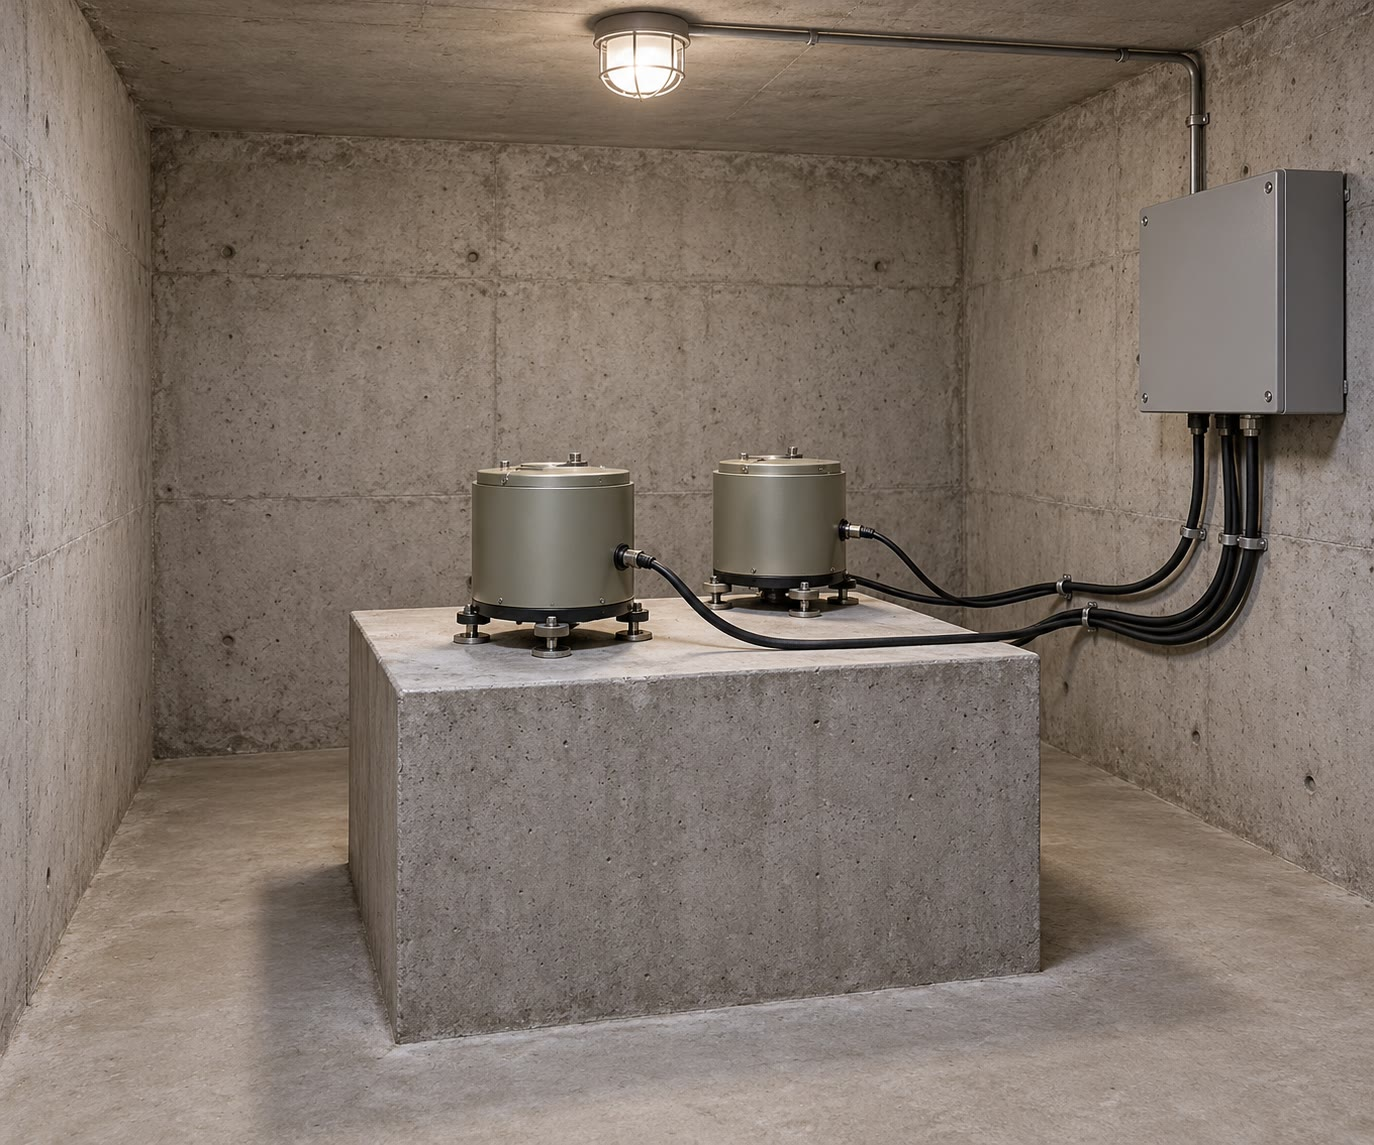
\includegraphics[width=0.58\linewidth]{images/book1/ai/g7-seismometer-vault.jpg}

{\small \omterm{def:g7:earthquakes:seismometer}{Sismômetros} numa sala subterrânea silenciosa, sobre um pilar de
concreto que se apoia na \omterm{def:g3:stones-pebbles-sand:rock}{rocha}, longe das estradas e das máquinas
(ilustração de uma cena genérica feita por IA).}
\label{fig:g7:earthquakes:vault}
\end{omfigure}

\section{Qual é o tamanho? Magnitude e intensidade}

Dois números diferentes descrevem um \omterm{def:g4:volcanoes-earthquakes-first-look:earthquake}{terremoto}, e eles muitas vezes são confundidos.

\begin{definition}[Magnitude]\label{def:g7:earthquakes:magnitude}
A \emph{magnitude}\index{magnitude} de um \omterm{def:g4:volcanoes-earthquakes-first-look:earthquake}{terremoto} mede o seu tamanho: a
energia liberada na origem. Ela é calculada a partir dos \omterm{def:g7:earthquakes:seismometer}{sismogramas}.
Cada \omterm{def:g4:volcanoes-earthquakes-first-look:earthquake}{terremoto} tem uma única magnitude, escrita com uma casa decimal,
como 6.3 ou 9.1.
\end{definition}

\begin{definition}[Intensidade]\label{def:g7:earthquakes:intensity}
A \emph{intensidade}\index{intensidade} de um \omterm{def:g4:volcanoes-earthquakes-first-look:earthquake}{terremoto} num lugar descreve
com que força o chão tremeu ali, a partir do que as pessoas sentiram e
dos estragos que elas viram. Ela é escrita em algarismos romanos, de I
(não sentido) a XII (destruição total). Um \omterm{def:g4:volcanoes-earthquakes-first-look:earthquake}{terremoto} tem muitas
intensidades: uma diferente em cada lugar.
\end{definition}

A escala de magnitude sobe rápido. Cada degrau de 1 na \omterm{def:g7:earthquakes:magnitude}{magnitude}
corresponde a ondas cerca de 10~vezes maiores no \omterm{def:g7:earthquakes:seismometer}{sismograma} e a cerca de
32~vezes mais energia liberada. Um \omterm{def:g4:volcanoes-earthquakes-first-look:earthquake}{terremoto} de \omterm{def:g7:earthquakes:magnitude}{magnitude}~8 libera cerca
de $32 \times 32 \approx 1000$ vezes mais energia que um de \omterm{def:g7:earthquakes:magnitude}{magnitude}~6.
% ledger: usgs:mag-energy

\begin{method}[Comparar duas magnitudes]\label{met:g7:earthquakes:magnitudes}
Para comparar a energia de dois \omterm{def:g4:volcanoes-earthquakes-first-look:earthquake}{terremotos}, conte os degraus inteiros
entre as suas \omterm{def:g7:earthquakes:magnitude}{magnitudes}, e multiplique por 32 uma vez para cada degrau:
1~degrau, 32~vezes; 2~degraus, cerca de 1000~vezes; 3~degraus, cerca de
32\,000~vezes.
\end{method}

\begin{example}[Magnitude 9 e magnitude 7]\label{ex:g7:earthquakes:nine-seven}
O \omterm{def:g4:volcanoes-earthquakes-first-look:earthquake}{terremoto} de 2004 ao largo de Sumatra teve uma \omterm{def:g7:earthquakes:magnitude}{magnitude} de 9.1. Um
\omterm{def:g4:volcanoes-earthquakes-first-look:earthquake}{terremoto} de \omterm{def:g7:earthquakes:magnitude}{magnitude}~7.1 é dois degraus menor: ele liberou cerca de
$32 \times 32 = 1024$, ou seja, cerca de 1000~vezes menos energia.
% ledger: usgs:largest, usgs:mag-energy
\end{example}

Os maiores \omterm{def:g4:volcanoes-earthquakes-first-look:earthquake}{terremotos} já medidos aconteceram todos onde uma \omterm{def:g7:plate-tectonics:plate}{placa} afunda
embaixo de outra: \omterm{def:g7:earthquakes:magnitude}{magnitude}~9.5 no Chile em 22~de~maio~de~1960, 9.2 no
Alasca em 1964, 9.1 ao largo de Sumatra em 2004 e 9.1 ao largo do \omterm{def:g1:landscapes-around-us:water}{litoral}
do Japão em 11~de~março~de~2011. Os grandes \omterm{def:g4:volcanoes-earthquakes-first-look:earthquake}{terremotos} são raros, e quanto
maiores, mais raros, como mostra o gráfico: a cada degrau a mais de
\omterm{def:g7:earthquakes:magnitude}{magnitude}, cerca de dez vezes menos.
% ledger: usgs:largest, data:usgs-comcat

\begin{omfigure}
\begin{tikzpicture}
  \begin{axis}[ybar, width=0.72\linewidth, height=5.4cm, bar width=22pt,
      ymode=log, log origin y=infty, ymin=0.01, ymax=600,
      xtick=data, xticklabels={6 a 6.9,7 a 7.9,8 a 8.9,9 ou mais},
      xlabel={magnitude}, ylabel={terremotos por ano},
      ytick={0.01,0.1,1,10,100}, yticklabels={0.01,0.1,1,10,100},
      tick label style={font=\scriptsize}, label style={font=\small},
      nodes near coords, point meta=explicit symbolic,
      nodes near coords style={font=\scriptsize}, enlarge x limits=0.18,
      axis x line*=bottom, axis y line*=left]
    \addplot[fill=omThm!45, draw=omThm!80!black] table[x=cls, y=per_year, meta=per_year] {figdata/out/grade-7-quake_counts.dat};
  \end{axis}
\end{tikzpicture}

{\small \omterm{def:g4:volcanoes-earthquakes-first-look:earthquake}{Terremotos} por ano, em média em 1976--2025, por \omterm{def:g7:earthquakes:magnitude}{magnitude}. A
escala vertical é especial: cada linha vale dez vezes a de baixo. Dados:
catálogo de \omterm{def:g4:volcanoes-earthquakes-first-look:earthquake}{terremotos} do U.S. Geological Survey (7\,031 \omterm{def:g4:volcanoes-earthquakes-first-look:earthquake}{terremotos} de
\omterm{def:g7:earthquakes:magnitude}{magnitude}~6 ou mais).}
% ledger: data:usgs-comcat (figdata/grade-7/quake_counts.py, main table)
\label{fig:g7:earthquakes:counts}
\end{omfigure}

A escala de intensidade não tem fórmula: é uma lista do que acontece. A
tabela a apresenta de forma resumida.
% ledger: usgs:mmi, usgs:mmi-page

\begin{center}
\small
\begin{tabular}{|c|p{0.8\linewidth}|}
\hline
\textbf{\omterm{def:g7:earthquakes:intensity}{intensidade}} & \textbf{o que se sente e o que se vê} \\
\hline
I & não sentido, a não ser por pouquíssimas pessoas \\
II & sentido só por algumas pessoas em repouso, sobretudo nos andares de cima; objetos pendurados podem balançar \\
III & sentido dentro de casa; parece a passagem de um caminhão \\
IV & sentido dentro de casa por muitos; louças, janelas e portas chacoalham \\
V & sentido por quase todos, muitos acordam; algumas louças e janelas se quebram \\
VI & sentido por todos, muitos se assustam; alguns móveis pesados se deslocam; estragos leves \\
VII & poucos estragos nos prédios bem construídos, muitos nos mal construídos; algumas chaminés se quebram \\
VIII & muitos estragos nos prédios comuns, alguns desabam em parte; chaminés e muros caem \\
IX & grandes estragos até nos prédios sólidos; prédios deslocados das suas fundações \\
X & a maioria dos prédios destruída junto com as fundações; trilhos entortados \\
XI & poucos prédios continuam de pé; pontes destruídas \\
XII & estragos totais; objetos lançados no ar \\
\hline
\end{tabular}
\end{center}
% ledger: usgs:mmi

A \omterm{def:g7:earthquakes:intensity}{intensidade}, em geral, é maior perto do \omterm{def:g7:earthquakes:focus}{epicentro} e diminui com a
distância. Mas ela também depende do terreno: a \omterm{def:g3:stones-pebbles-sand:rock}{rocha} sólida é a que
treme menos, a \omterm{def:g3:stones-pebbles-sand:sand}{lama} mole é a que treme mais. Uma cidade construída sobre
terreno mole pode tremer mais forte que outra cidade mais perto do
\omterm{def:g7:earthquakes:focus}{epicentro}, mas construída sobre \omterm{def:g3:stones-pebbles-sand:rock}{rocha}.
% ledger: usgs:mag-energy

\begin{omfigure}
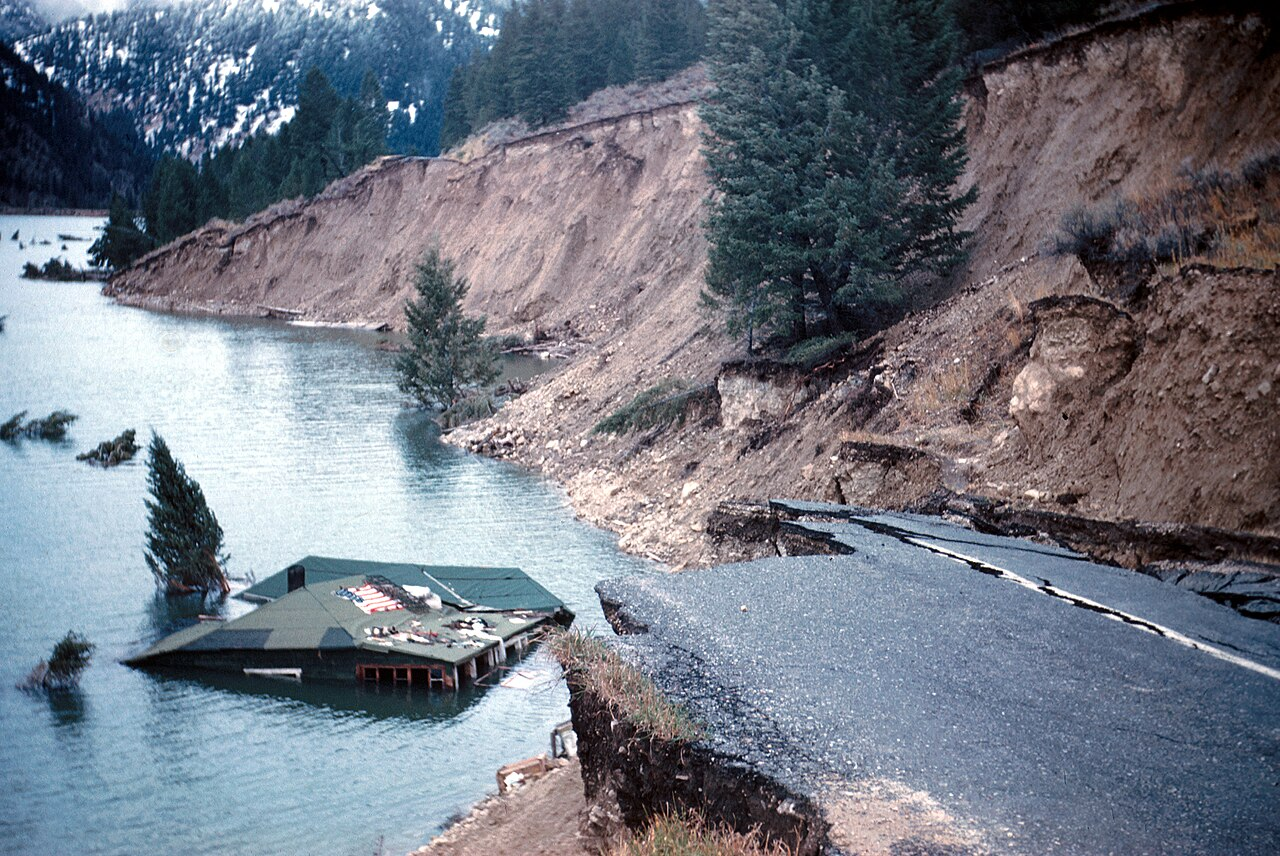
\includegraphics[width=0.6\linewidth]{images/book1/g7-hebgen-road.jpg}

{\small Depois do \omterm{def:g4:volcanoes-earthquakes-first-look:earthquake}{terremoto} de Hebgen Lake, em Montana (Estados Unidos),
em agosto~de~1959: a estrada ao longo do \omterm{def:g1:landscapes-around-us:water}{lago} escorregou para dentro da
água, e um hotel acabou quase embaixo d'água. Estragos assim são a marca
de uma \omterm{def:g7:earthquakes:intensity}{intensidade} alta. Fotografia: I.~J. Witkind, U.S. Geological
Survey (domínio público, via Wikimedia Commons).}
% ledger: commons:hebgen-road, usgs:mmi
\label{fig:g7:earthquakes:hebgen}
\end{omfigure}

\section{Os tsunamis}

\begin{definition}[Tsunami]\label{def:g7:earthquakes:tsunami}
Um \emph{tsunami}\index{tsunami} é uma série de ondas do \omterm{def:g2:water-on-earth:ocean}{mar} provocadas
por um movimento repentino do fundo do \omterm{def:g2:water-on-earth:ocean}{mar} --- em geral um \omterm{def:g4:volcanoes-earthquakes-first-look:earthquake}{terremoto}
embaixo do \omterm{def:g2:water-on-earth:ocean}{mar}, às vezes uma \omterm{def:g4:volcanoes-earthquakes-first-look:eruption}{erupção} ---, que podem atravessar \omterm{def:g2:water-on-earth:ocean}{oceanos}
inteiros e inundar os \omterm{def:g1:landscapes-around-us:water}{litorais}.
\end{definition}

Quando uma \omterm{def:g7:earthquakes:fault}{falha} embaixo do \omterm{def:g2:water-on-earth:ocean}{mar} se rompe, o fundo do \omterm{def:g2:water-on-earth:ocean}{mar} sobe ou desce de
repente, e levanta ou abaixa toda a coluna de água acima dele. A água se espalha em ondas. Em pleno \omterm{def:g2:water-on-earth:ocean}{oceano} profundo, um \omterm{def:g7:earthquakes:tsunami}{tsunami}
surpreende: ele raramente passa de um metro de altura, e os navios nem
percebem quando ele passa por baixo deles. Mas ele é rápido: mais de
\qty{800}{km/h}, tão rápido quanto um avião a jato. Quando chega às águas
rasas perto do \omterm{def:g1:landscapes-around-us:water}{litoral}, ele desacelera para 30 ou \qty{50}{km/h} ---
ainda mais rápido do que qualquer pessoa consegue correr --- e fica mais
alto. A maioria dos \omterm{def:g7:earthquakes:tsunami}{tsunamis} tem menos de \qty{3}{m} de altura no
\omterm{def:g1:landscapes-around-us:water}{litoral}; os maiores passam de \qty{30}{m}. A primeira onda nem sempre é a
maior, e as ondas podem continuar chegando durante horas.
% ledger: nws:tsunami-speed, nws:tsunami-safety

\begin{omfigure}
\begin{tikzpicture}[font=\small, x=1cm, y=1cm]
  % sea floor profile: deep ocean on the left, shelf and coast on the right
  \fill[omSea!35] (0,0) -- (13.2,0) -- (13.2,-0.2) -- (11.4,-0.45) -- (10.2,-1.0) -- (8.8,-2.6) -- (0,-2.6) -- cycle;
  \fill[brown!35] (0,-2.6) -- (8.8,-2.6) -- (10.2,-1.0) -- (11.4,-0.45) -- (13.2,-0.2) -- (13.2,0.5) -- (14.2,1.0) -- (14.2,-3.3) -- (0,-3.3) -- cycle;
  % the broken fault under the sea, at left; one block lifted
  \draw[very thick, red!70!black] (1.9,-3.3) -- (2.3,-2.6);
  \draw[-{Stealth[length=2mm]}, thick] (2.75,-3.1) -- (2.75,-2.75);
  \node[anchor=north west, font=\footnotesize, red!70!black] at (0.1,-3.35) {a falha se rompe, o fundo do mar dá um salto};
  % wave: low and long in the deep ocean, short and tall near the coast
  \draw[blue!70!black, thick] (0,0) .. controls (1.2,0.18) and (2.2,0.18) .. (3.4,0)
     -- (5.0,0) .. controls (5.8,0.12) and (6.6,0.12) .. (7.4,0) -- (10.6,0)
     .. controls (11.0,0.55) and (11.6,0.9) .. (12.1,0) -- (13.2,0);
  \node[align=center, font=\footnotesize] at (2.0,0.85) {oceano profundo: cerca de 1 m de altura,\\mais de 800 km/h};
  \node[align=center, font=\footnotesize] at (11.1,1.55) {perto do litoral: mais lento\\(30 a 50 km/h), muito mais alto};
  \draw[-{Stealth[length=2.5mm]}, thick, blue!70!black] (4.4,0.45) -- (6.4,0.45);
  \node[font=\footnotesize] at (6.0,-1.5) {milhares de metros de profundidade};
  \node[font=\footnotesize] at (12.0,-0.75) {raso};
\end{tikzpicture}

{\small Um \omterm{def:g7:earthquakes:tsunami}{tsunami} atravessando o \omterm{def:g2:water-on-earth:ocean}{oceano} (um desenho, fora de escala: a
altura da onda está muito exagerada). Ele é baixo e muito rápido sobre o
\omterm{def:g2:water-on-earth:ocean}{oceano} profundo; ele desacelera e cresce nas águas rasas perto do
\omterm{def:g1:landscapes-around-us:water}{litoral}.}
% ledger: nws:tsunami-speed
\label{fig:g7:earthquakes:tsunami}
\end{omfigure}

\begin{example}[De Sumatra ao Sri Lanka]\label{ex:g7:earthquakes:colombo}
Colombo, a maior cidade do Sri Lanka, fica a cerca de \qty{1830}{km} do
\omterm{def:g7:earthquakes:focus}{epicentro} do \omterm{def:g4:volcanoes-earthquakes-first-look:earthquake}{terremoto} de 2004. A \qty{800}{km/h}, um \omterm{def:g7:earthquakes:tsunami}{tsunami} percorre
essa distância em $1830 \div 800 \approx 2.3$~horas, ou seja, cerca de
2~horas e 17~minutos. Ninguém no Sri Lanka sentiu o \omterm{def:g4:volcanoes-earthquakes-first-look:earthquake}{terremoto}: a onda
chegou sem nenhum aviso além do próprio \omterm{def:g2:water-on-earth:ocean}{mar}.
% ledger: nws:tsunami-speed, usgs:largest (distance and time in figdata/grade-7/quake_counts.py, part tsunami)
\end{example}

\begin{remark}[O aviso que o mar dá]\label{rem:g7:earthquakes:natural-warning}
% ledger: nws:tsunami-natural-warning, nws:tsunami-speed, shakeout:dch
Num \omterm{def:g1:landscapes-around-us:water}{litoral}, três sinais podem anunciar um \omterm{def:g7:earthquakes:tsunami}{tsunami}: um \omterm{def:g4:volcanoes-earthquakes-first-look:earthquake}{terremoto} forte ou
longo; o \omterm{def:g2:water-on-earth:ocean}{mar} se comportando de um jeito estranho --- uma \omterm{def:g5:water-shapes-the-land:flood}{inundação}
repentina, ou a água recuando para longe da praia e mostrando o fundo do
\omterm{def:g2:water-on-earth:ocean}{mar}, como numa maré muito baixa; ou um estrondo forte vindo do \omterm{def:g2:water-on-earth:ocean}{oceano}.
Durante o tremor, proteja-se como você aprendeu (abaixe-se, proteja-se,
segure-se). Depois, não espere um alerta oficial: vá o mais alto, ou o
mais longe terra adentro, que você puder, imediatamente. Um \omterm{def:g7:earthquakes:tsunami}{tsunami} vindo
de um \omterm{def:g4:volcanoes-earthquakes-first-look:earthquake}{terremoto} próximo pode chegar em poucos minutos.
\end{remark}


\section{Exercícios}

\begin{exercise}[$\star$]\label{exo:g7:earthquakes:1}
Ligue cada palavra ao seu significado: \omterm{def:g7:earthquakes:fault}{falha}; \omterm{def:g7:earthquakes:focus}{foco}; \omterm{def:g7:earthquakes:focus}{epicentro};
\omterm{def:g7:earthquakes:seismometer}{sismômetro}; \omterm{def:g7:earthquakes:magnitude}{magnitude}; \omterm{def:g7:earthquakes:intensity}{intensidade}. (a) O lugar embaixo da terra onde o
deslizamento começa. (b) Com que força o chão tremeu num lugar. (c) Uma
ruptura nas \omterm{def:g3:stones-pebbles-sand:rock}{rochas} ao longo da qual os dois lados se deslocaram. (d) O
ponto da superfície acima do \omterm{def:g7:earthquakes:focus}{foco}. (e) O tamanho de um \omterm{def:g4:volcanoes-earthquakes-first-look:earthquake}{terremoto}, um
número para cada \omterm{def:g4:volcanoes-earthquakes-first-look:earthquake}{terremoto}. (f) Um instrumento que registra o tremor do
chão.
\end{exercise}

\begin{exercise}[$\star$]\label{exo:g7:earthquakes:2}
O \omterm{def:g7:earthquakes:focus}{foco} de um \omterm{def:g4:volcanoes-earthquakes-first-look:earthquake}{terremoto} fica a \qty{30}{km} bem embaixo de uma aldeia.
(a) Onde fica o \omterm{def:g7:earthquakes:focus}{epicentro}? (b) A que distância a aldeia fica do \omterm{def:g7:earthquakes:focus}{foco}?
(c) Uma segunda aldeia fica a \qty{40}{km} do \omterm{def:g7:earthquakes:focus}{epicentro}. A sua
\omterm{def:g7:earthquakes:intensity}{intensidade} em geral vai ser maior ou menor que na primeira aldeia? Por
quê?
\end{exercise}

\begin{exercise}[$\star$]\label{exo:g7:earthquakes:3}
\omterm{def:g7:earthquakes:magnitude}{Magnitude} ou \omterm{def:g7:earthquakes:intensity}{intensidade}? (a) ``O \omterm{def:g4:volcanoes-earthquakes-first-look:earthquake}{terremoto} mediu 6.8.'' (b) ``Na nossa
rua, todas as louças caíram e uma chaminé se quebrou.'' (c) ``Foi VI na
cidade e IV nas aldeias dos morros.'' (d) ``Ele liberou 32~vezes mais
energia que o do ano passado.''
\end{exercise}

\begin{exercise}[$\star$]\label{exo:g7:earthquakes:4}
Verdadeiro ou falso? Corrija as falsas. (a) Os cientistas conseguem dizer
com uma semana de antecedência quando um \omterm{def:g4:volcanoes-earthquakes-first-look:earthquake}{terremoto} vai acontecer. (b) Em
pleno \omterm{def:g2:water-on-earth:ocean}{oceano}, um \omterm{def:g7:earthquakes:tsunami}{tsunami} é uma enorme parede de água. (c) Um \omterm{def:g4:volcanoes-earthquakes-first-look:earthquake}{terremoto}
tem uma única \omterm{def:g7:earthquakes:magnitude}{magnitude}, mas muitas \omterm{def:g7:earthquakes:intensity}{intensidades}. (d) A maioria dos
grandes \omterm{def:g4:volcanoes-earthquakes-first-look:earthquake}{terremotos} acontece perto dos \omterm{def:g7:plate-tectonics:plate-boundary}{limites de placas}.
\end{exercise}

\begin{exercise}[$\star\star$]\label{exo:g7:earthquakes:5}
Use o gráfico dos \omterm{def:g4:volcanoes-earthquakes-first-look:earthquake}{terremotos} por ano. (a) Cerca de quantos \omterm{def:g4:volcanoes-earthquakes-first-look:earthquake}{terremotos} de
\omterm{def:g7:earthquakes:magnitude}{magnitude} 6 a 6.9 acontecem num ano? E de \omterm{def:g7:earthquakes:magnitude}{magnitude} 7 a 7.9? (b) Quantas
vezes menos numerosos são os segundos que os primeiros? (c) Some as três
barras a partir de 7: cerca de quantos \omterm{def:g4:volcanoes-earthquakes-first-look:earthquake}{terremotos} de \omterm{def:g7:earthquakes:magnitude}{magnitude} 7 ou mais
acontecem num ano? (d) O gráfico indica 0.04 por ano para a \omterm{def:g7:earthquakes:magnitude}{magnitude} 9
ou mais. Quantos isso dá em 50~anos?
\end{exercise}

\begin{exercise}[$\star\star$]\label{exo:g7:earthquakes:6}
Use o método para comparar \omterm{def:g7:earthquakes:magnitude}{magnitudes}. (a) Quantas vezes mais energia um
\omterm{def:g4:volcanoes-earthquakes-first-look:earthquake}{terremoto} de \omterm{def:g7:earthquakes:magnitude}{magnitude} 7 libera que um de \omterm{def:g7:earthquakes:magnitude}{magnitude} 6? (b) E um de
\omterm{def:g7:earthquakes:magnitude}{magnitude} 8 que um de \omterm{def:g7:earthquakes:magnitude}{magnitude} 6? (c) Quantas vezes maiores são as suas
ondas no \omterm{def:g7:earthquakes:seismometer}{sismograma}, para a mesma distância, entre a \omterm{def:g7:earthquakes:magnitude}{magnitude} 6 e a 8?
\end{exercise}

\begin{exercise}[$\star\star$]\label{exo:g7:earthquakes:7}
Use \qty{8}{km} para cada segundo de atraso entre as ondas mais rápidas e
as mais lentas. (a) Uma estação registra um atraso de \qty{5}{s}. A que
distância foi o \omterm{def:g4:volcanoes-earthquakes-first-look:earthquake}{terremoto}? (b) Outra registra \qty{25}{s}. (c) Um
\omterm{def:g4:volcanoes-earthquakes-first-look:earthquake}{terremoto} aconteceu a \qty{120}{km} de uma estação: que atraso a estação
vai ler? (d) Por que uma única estação não consegue dizer onde fica o
\omterm{def:g7:earthquakes:focus}{epicentro}?
\end{exercise}

\begin{exercise}[$\star\star$]\label{exo:g7:earthquakes:8}
Use a tabela das \omterm{def:g7:earthquakes:intensity}{intensidades}. Dê a \omterm{def:g7:earthquakes:intensity}{intensidade} de cada relato.
(a) ``Sentido por quase todo mundo; nós acordamos e dois copos se
quebraram.'' (b) ``Só a minha avó, descansando no andar de cima, sentiu;
a lâmpada balançou.'' (c) ``Muros e chaminés caíram; várias casas
desabaram em parte.'' (d) O mesmo \omterm{def:g4:volcanoes-earthquakes-first-look:earthquake}{terremoto} deu os relatos (a) e (c).
Explique como isso é possível.
\end{exercise}

\begin{exercise}[$\star\star$]\label{exo:g7:earthquakes:9}
Dos 7\,031 \omterm{def:g4:volcanoes-earthquakes-first-look:earthquake}{terremotos} de \omterm{def:g7:earthquakes:magnitude}{magnitude}~6 ou mais de 1976--2025, 5\,561
tiveram o seu \omterm{def:g7:earthquakes:focus}{foco} a menos de \qty{70}{km} de profundidade. (a) Quantos
tiveram um \omterm{def:g7:earthquakes:focus}{foco} mais profundo? (b) Que porcentagem isso representa?
Arredonde para o número inteiro mais próximo. (c) Os profundos acontecem
onde uma \omterm{def:g7:plate-tectonics:plate}{placa} afunda embaixo de outra. Explique por que eles podem
começar tão fundo ali.
\end{exercise}

\begin{exercise}[$\star\star$]\label{exo:g7:earthquakes:10}
Malé, a capital das Maldivas, fica a cerca de \qty{2500}{km} do
\omterm{def:g7:earthquakes:focus}{epicentro} do \omterm{def:g4:volcanoes-earthquakes-first-look:earthquake}{terremoto} de 2004. (a) A \qty{800}{km/h}, quanto tempo o
\omterm{def:g7:earthquakes:tsunami}{tsunami} levou para chegar lá? Dê as horas e os minutos. (b) Quanto tempo
depois de Colombo (2~horas e 17~minutos) ele chegou? (c) Com atrasos
assim, por que um sistema de alerta poderia ter salvado muitas vidas?
\end{exercise}

\begin{exercise}[$\star\star\star$]\label{exo:g7:earthquakes:11}
Um \omterm{def:g7:earthquakes:tsunami}{tsunami} atravessa \qty{400}{km} de \omterm{def:g2:water-on-earth:ocean}{oceano} profundo a \qty{800}{km/h},
e depois os últimos \qty{20}{km} de águas rasas a \qty{40}{km/h}.
(a) Quantos minutos ele leva na parte profunda? (b) E na parte rasa?
(c) Quanto dura a viagem inteira? (d) O que é surpreendente nas suas
respostas? (e) Por que a onda fica mais alta quando desacelera?
\end{exercise}

\begin{exercise}[$\star\star\star$]\label{exo:g7:earthquakes:12}
(a) Quantas vezes mais energia um \omterm{def:g4:volcanoes-earthquakes-first-look:earthquake}{terremoto} de \omterm{def:g7:earthquakes:magnitude}{magnitude} 9 libera que um
de \omterm{def:g7:earthquakes:magnitude}{magnitude} 6? (b) Todo ano, há cerca de 127 \omterm{def:g4:volcanoes-earthquakes-first-look:earthquake}{terremotos} de \omterm{def:g7:earthquakes:magnitude}{magnitude} 6 a
6.9. Suponha que cada um deles libera a energia de uma \omterm{def:g7:earthquakes:magnitude}{magnitude} 6.
Quantos anos deles são necessários para liberar a energia de um único
\omterm{def:g4:volcanoes-earthquakes-first-look:earthquake}{terremoto} de \omterm{def:g7:earthquakes:magnitude}{magnitude}~9? (c) O que isso diz sobre a parte da energia
levada pelos maiores \omterm{def:g4:volcanoes-earthquakes-first-look:earthquake}{terremotos}?
\end{exercise}

\section{Problema: Onde o chão tremeu?}

\begin{problem}[{Problema de fim de semana --- três estações registram um
terremoto embaixo do mar, o epicentro é encontrado no mapa, e a cidade de
Port Hale recebe o alerta antes de o tsunami chegar}]
\label{pb:g7:earthquakes:1}
% ledger: nws:tsunami-speed, usgs:seismograph, data:prem (figdata/grade-7/epicentre.py)
Um \omterm{def:g4:volcanoes-earthquakes-first-look:earthquake}{terremoto} acontece embaixo do \omterm{def:g2:water-on-earth:ocean}{mar} de um \omterm{def:g1:landscapes-around-us:water}{litoral} inventado. Três
estações de \omterm{def:g7:earthquakes:seismometer}{sismômetros}, A, B e C, ficam em terra; a cidade de Port Hale
fica numa ilha (\omterm{def:g2:drawing-to-map:map}{mapa} abaixo; um quadrado vale \qty{20}{km}). Nessa região,
cada segundo de atraso entre as ondas mais rápidas e as mais lentas
corresponde a \qty{8}{km}. As estações registram:

\begin{center}
\small
\begin{tabular}{|c|c|c|}
\hline
\textbf{estação} & \textbf{chegada das ondas rápidas} & \textbf{chegada das ondas lentas} \\
\hline
A & 10:15:25 & 10:15:45 \\
B & 10:15:16 & 10:15:29 \\
C & 10:15:19 & 10:15:34 \\
\hline
\end{tabular}
\end{center}

\medskip
\noindent\textbf{Parte I --- Três estações.}\par\nopagebreak
\begin{enumerate}[beginpenalty=10000]
  \item Para cada estação, encontre o atraso entre as duas chegadas, em
        segundos.
  \item Que estação fica mais perto do \omterm{def:g4:volcanoes-earthquakes-first-look:earthquake}{terremoto}? Como você pode saber
        sem fazer nenhuma conta?
  \item Encontre a distância de cada estação até o \omterm{def:g4:volcanoes-earthquakes-first-look:earthquake}{terremoto}.
  \item Só a distância da estação A não diz onde foi o \omterm{def:g4:volcanoes-earthquakes-first-look:earthquake}{terremoto}.
        Descreva todos os lugares que ficam a essa distância de A.
\end{enumerate}

\begin{center}
\begin{tikzpicture}
  \begin{axis}[axis equal image, width=12cm, xmin=-60, xmax=360, ymin=-200, ymax=260,
      xtick={-60,-40,...,360}, ytick={-200,-180,...,260}, xticklabels={}, yticklabels={},
      major tick length=0pt,
      axis background/.style={fill=omSea!25}, clip mode=individual]
    \addplot[fill=omLithAlluv, draw=black!50, line width=0.4pt] table[x=x, y=y] {figdata/out/grade-7-epicentre-p-west.dat};
    \addplot[fill=omLithAlluv, draw=black!50, line width=0.4pt] table[x=x, y=y] {figdata/out/grade-7-epicentre-p-north.dat};
    \addplot[fill=omLithAlluv, draw=black!50, line width=0.4pt] table[x=x, y=y] {figdata/out/grade-7-epicentre-p-island.dat};
    % the grid over land and sea, drawn before the labels
    \pgfplotsinvokeforeach{-40,-20,...,340}{\draw[black!15] (axis cs:#1,-200) -- (axis cs:#1,260);}
    \pgfplotsinvokeforeach{-180,-160,...,240}{\draw[black!15] (axis cs:-60,#1) -- (axis cs:360,#1);}
    \addplot[only marks, mark=triangle*, mark size=3.2pt, black,
        nodes near coords, point meta=explicit symbolic,
        nodes near coords style={font=\small\bfseries, anchor=south west}]
      table[x=x, y=y, meta=name] {figdata/out/grade-7-epicentre-p-stations.dat};
    \addplot[only marks, mark=square*, mark size=2.4pt, red!70!black,
        nodes near coords, point meta=explicit symbolic,
        nodes near coords style={font=\small, anchor=north east, fill=omSea!25, inner sep=1pt}]
      table[x=x, y=y, meta=name] {figdata/out/grade-7-epicentre-p-town.dat};
    \draw[-{Stealth[length=2.5mm]}, line width=0.8pt] (axis cs:330,200) -- (axis cs:330,245);
    \node[font=\scriptsize\bfseries, anchor=north] at (axis cs:330,200) {N};
    \node[font=\scriptsize, anchor=west, fill=omLithAlluv, inner sep=1pt] at (axis cs:170,240) {1 quadrado = 20 km};
    \fill (axis cs:-60,-200) circle (1.5pt);
    \node[font=\small\bfseries, anchor=north east] at (axis cs:-60,-200) {O};
  \end{axis}
\end{tikzpicture}
\end{center}
% ledger: (invented map: figdata/grade-7/epicentre.py, parts p-west, p-north, p-island, p-stations, p-town)

\medskip
\noindent\textbf{Parte II --- Encontrar o epicentro.}\par\nopagebreak
\begin{enumerate}[resume, beginpenalty=10000]
  \item Um quadrado vale \qty{20}{km}. Quantos quadrados mede o raio de
        cada círculo?
  \item Ponha o canto O embaixo, à esquerda do \omterm{def:g2:drawing-to-map:map}{mapa}. A estação C fica
        3~quadrados a leste e 14.5~quadrados ao norte de O; andando
        6~quadrados (\qty{120}{km}) bem para o leste a partir de C, você
        chega a um ponto~E. Verifique no \omterm{def:g2:drawing-to-map:map}{mapa} que E também fica nos
        círculos de A e de B: é o \omterm{def:g7:earthquakes:focus}{epicentro}. Quantos quadrados a leste e
        ao norte de O ele fica?
  \item O \omterm{def:g7:earthquakes:focus}{epicentro} fica em terra ou embaixo do \omterm{def:g2:water-on-earth:ocean}{mar}? Por que isso
        importa?
  \item A \omterm{def:g7:earthquakes:magnitude}{magnitude} foi de 7.4. Quantas vezes mais energia que um
        \omterm{def:g4:volcanoes-earthquakes-first-look:earthquake}{terremoto} de \omterm{def:g7:earthquakes:magnitude}{magnitude}~6.4 ele liberou?
\end{enumerate}

\medskip
\noindent\textbf{Parte III --- A onda chega ao litoral.}\par\nopagebreak
\begin{enumerate}[resume, beginpenalty=10000]
  \item No \omterm{def:g2:drawing-to-map:map}{mapa}, Port Hale fica a 12~quadrados do \omterm{def:g7:earthquakes:focus}{epicentro}. Quantos
        quilômetros isso dá?
  \item A \qty{800}{km/h}, quantos minutos o \omterm{def:g7:earthquakes:tsunami}{tsunami} leva para chegar a
        Port Hale?
  \item Localizar o \omterm{def:g4:volcanoes-earthquakes-first-look:earthquake}{terremoto} e mandar o alerta leva 5~minutos depois do
        começo do tremor. Quanto tempo depois do \omterm{def:g4:volcanoes-earthquakes-first-look:earthquake}{terremoto} o alerta chega
        a Port Hale?
  \item Quantos minutos os moradores de Port Hale têm para chegar a um
        lugar alto antes de o \omterm{def:g7:earthquakes:tsunami}{tsunami} chegar?
\end{enumerate}
\end{problem}
